\section{Zielsetzung}
\label{sec:zielsetzung}

    In diesem Versuch soll das Experiment, in welchem die Physiker James Franck und Gustav Hertz im Jahr 1914 die Energieübertragung bei Stößen von Elektronen mit 
    Atomen untersucht haben, näher betrachtet werden. Dazu wird der Versuchsaufbau nachempfunden und die Messungen der Physiker wiederholt. Es wird die 
    Energiedifferenz zwischen dem ersten angeregten Zustand und dem Grundzustand, die Energieverteilung der Elektronen und die Ionisationsenergie des 
    Quecksilberatoms ermittelt werden. 

\section{Theorie}
\label{sec:Theorie}

    Der Franck-Herzt-Versuch gehört zu einer dreijährigen Messreihe der Physiker James Franck und Gustav Hertz. In dem Elektronenstoßexperiment gelingt es einer
    Anregungsenergie des Quersilberatoms zu ermitteln und einen Zusammenhang von dieser mit der Wellenlänge des Photons, welches beim Zurückgehen in den 
    Grundzustand emittiert wird. Damit können im gewissen Maße die Bohr'schen Postulate, welche 1913 von Niels Bohr aufgestellt wurden, experimentell verifiziert 
    werden und die Elektronenhülle besser verstanden werden. \\
    
    \noindent Bei einem Elektronenstoßexperiment werden Atome mit Elektronen beschossen und aus den Energiedifferenzen der Elektronen Rückschlüsse gezogen. 
    In dem Franck-Hertz-Versuch werden Quecksilberatome mit Elektronen verschiedener Energien beschossen und stoße elastisch und inelastisch miteinander. 


\subsection{Aufbau und Ablauf des Franck-Hertz-Versuches}

    


    \begin{figure}
         \centering 
         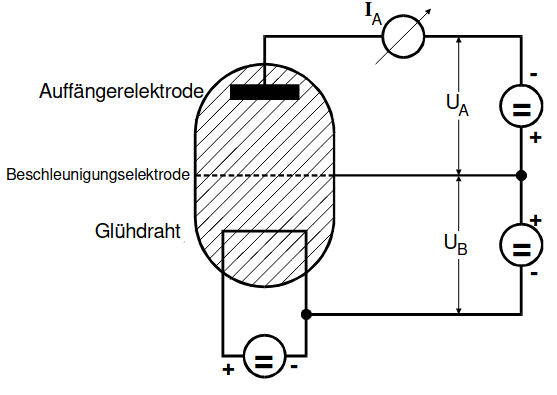
\includegraphics[width=\textwidth]{bilder/prinzipieller_aufbau.png}
         \caption{Prinzipieller Aufbau des Franck-Hertz-Versuches \cite{anleitung}.}
         \label{fig:prinzipieller_aufbau}
    \end{figure}

    \begin{figure}
        \centering 
        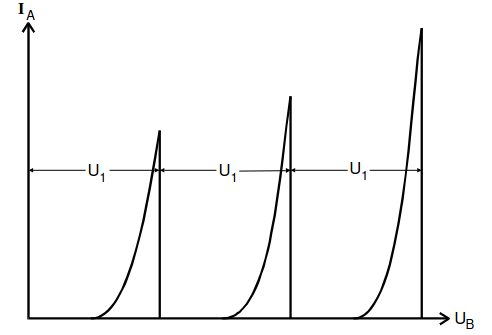
\includegraphics[width=\textwidth]{bilder/idealer_Ub_Ia.png}
        \caption{Idealisierter Zusammenhang zwischen dem Strom des Gegenfeldes $I_{\text{A}}$ und der Beschleunigungsspannung $U_{\text{B}}$ \cite{anleitung}. }
        \label{fig:idealisiert}
    \end{figure}

\subsection{Einflüsse auf die Gestalt der Franck-Hertz-Kurve}

    \begin{figure}
        \centering 
        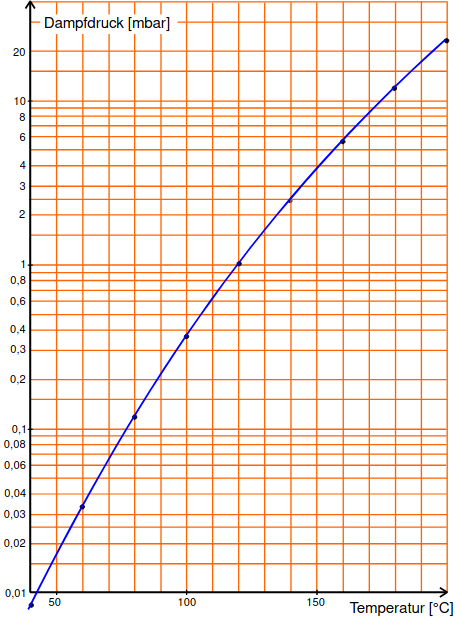
\includegraphics[width=0.7\textwidth]{bilder/Dampfdruckkurve.png}
        \caption{Dampfdruckkurve des Quecksilbers \cite{anleitung}.}
        \label{fig:dampfdruckkurve}
    \end{figure}

\subsection{Aufbau der Hg-Elektronenhülle}


    \begin{figure}
        \centering 
        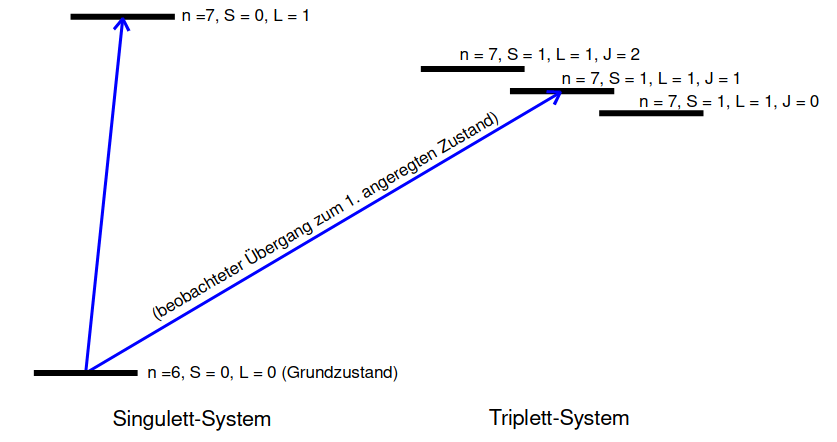
\includegraphics[width=0.8\textwidth]{bilder/Termschema.png}
        \caption{Ein nicht maßstäbliches Termschema eines Hg-Atoms \cite{anleitung}.}
        \label{fig:termschema}
    \end{figure}

